\chapter{A Metamodelling Facility}
\label{xmfchapter}

\section{Introduction}

In order to be able to construct semantically rich models of
languages, a facility that fully supports language definition is
required. This is known as a {\em metamodelling facility}. A
metamodelling facility should provide the ability to capture the
key features of a language, including its syntax and semantics in
a unified and platform independent way, along with support for
other important language design requirements such as extensibility
and executability.

This chapter gives a brief introduction to a metamodelling
facility called XMF (eXecutable Metamodelling Facility). XMF
extends existing standards such as MOF, OCL and QVT with rich
executable metamodelling capabilities. It provides a number of
languages for metamodelling, all based around a core executable
meta-architecture and metamodelling framework.

XMF will form the foundation for exploring metamodelling
throughout the rest of this book.

\section{Requirements of a Metamodelling Facility}

Before introducing XMF, it is important to understand some of the
key requirements of a metamodelling facility.

Firstly, as discussed in the previous chapter, a metamodelling
facility should provide metamodelling languages that can capture
all the essential features of a language. They should include
languages that can capture the abstract syntax, concrete syntax
and semantics of a language. In addition, it should provide
facilities for manipulating metamodels, including the ability to
map them to other metamodels and extend metamodels to support new
language definitions.

Secondly, it should provide a meta-architecture in which the
metamodelling languages (including their semantics) are themselves
described in terms of a core metamodelling language. This ensures
that the languages are self defined and complete, and enables
their definitions to be readily reused to create new language
definitions.

Finally, to gain maximum flexibility, a metamodelling facility
must be platform independent. In other words, its metamodels
should be self sufficient and independent of implementation
specific descriptions of the language being modelled. Thus,
reliance on the implementation of the language's behaviour in a
programming language or the assumption that there will be an
external database that manages object creation and persistence is
completely avoided.

\subsection{XMF}

XMF aims to provide a rich environment for language design that
supports the key requirements of a metamodelling facility. It
combines and extends a number of standard object-oriented
modelling facilities to provide a minimal, but expressive,
platform independent language for metamodelling. It includes the
following features:

\begin{itemize}

\item Support for core OO modelling concepts such as packages, classes, and
associations to describe language concepts and their relationship to one another.

\item A constraint language, which can used to describe well-formedness rules.

\item A set of action primitives, which can be used to capture the behavioural
semantics of a language and for manipulating metamodels. This
turns it into a meta-programming language.

\item A concrete syntax language which can be used to model the concrete
syntax of any modelling language.

\item A generic metamodel framework, which supports standard plug-points
and machinery for expressing model element instantiation,
execution, expression evaluation and reflection.

\item Conformance to the golden-braid metamodel architecture
described in section \ref{goldenbraid}, ensuring that the
language, including its semantics is completely self described.

\item A collection of richer metamodelling facilities. In particular,
languages for expressing mappings (both uni-directional and
bi-directional) between metamodels.

\end{itemize}

The following sections present an overview of the key features of
XMF. This is not a full definition, but will reference fuller
descriptions of the components of the language where appropriate.

\section{XMF Features}

\subsection{Core OO Modelling Concepts}
\label{coreconcepts}

XMF provides the standard OO modelling concepts that are supported
by MOF and UML, including packages, classes and associations.
These are visualised using class diagrams. Figure
\ref{classDiagram} shows an example of a class diagram of a simple
model consisting of a package with a number of classes and
associations. This model describes a simple StateMachine, where a
StateMachine contains States and Transitions, and Transitions have
source and target states.

\begin{figure}[htb]
\begin{center}
\includegraphics[width=10cm]{XMF/figures/classdiagramexample}
\caption{An example of a class diagram}
\label{classDiagram}
\end{center}
\end{figure}

Note that associations are defined in terms of attributes. Thus, a
uni-directional association (with a single arrow head) is visual
syntax for an attribute of the target type belonging to the source
class. A bi-directional association (with no arrow heads) is
visual syntax for a pair of attributes plus a constraint that
ensures they are inverses of one another.

XMF also provides a concrete syntax for packages and classes. The
equivalent concrete representation of the StateMachine class
diagram shown in figure \ref{classDiagram} is shown below.

\begin{lstlisting}
1  @Package StateMachines
2    @Class isAbstract Named
3      @Attribute name : String end
4    end
5    @Class StateMachine extends Named
6      @Attribute startName : String end
7      @Attribute states : Set(State) end
8      @Attribute transitions : Set(Transition) end
9    end
10   @Class State extends Named
11   end
12   @Class Transition
13     @Attribute sourceName : String end
14     @Attribute targetName : String end
15   end
16 end
\end{lstlisting}Line 1 shows the start of a package named StateMachines, which
contains all the sub-definitions relating to StateMachines.

Line 2 contains the start of a class definition for the class
Named,  which is an abstract class for a named element. Line 5 is
the start of the definition of the StateMachine class. It defines
three attributes. The first attribute is the name of the starting
state of the StateMachine. The other two attributes are states and
transitions, and their types are Set(State) and Set(Transition).
These types correspond to the "*" multiplicity of the equivalent
association ends in the class diagram.

Lines 10 and 12 are the start of the State and Transition class
definitions. The State class specialises the class Named, and
therefore inherits a name attribute. A Transition has two
attributes sourceName and targetName, which are the names of its
source and target states.

As chapter \ref{concretechapter} will show, the concrete
representation of a modelling language should be clearly
distinguished from its abstract syntax representation. Here, two
different concrete syntaxes are being used to capture the same
information.

\subsection{Imports}

Just as in UML and MOF, a package can be imported into another
package. The result is that all referenceable elements in the
imported package can be referenced by elements in the importing
package. Consider the following package:


\begin{lstlisting}
@Package X
  @Class Y end
end

@Package A imports X
  @Class B
    @Attribute b : Y end
  end
end
\end{lstlisting}
Because the package A imports the package X, elements in the
package X can be referenced without the need to provide a full
path name.

\subsection{Constraints}

It is often necessary to state well-formedness rules about
concepts in a model. These rules are often made informally, for
example in the context of figure \ref{classDiagram} it might be
useful to specify that \emph{all transitions have unique names}. A
constraint language provides a means of succinctly and
unambiguously expressing complex well-formedness rules. The
well-formedness rule mentioned above can be added to the class
StateMachine as follows:


\begin{lstlisting}
context StateMachine
  @Constraint NoTwoTransitionsWithTheSameName
    transitions->forAll(t1 |
      transitions->forAll(t2 |
        t1.name = t2.name implies t1 = t2))
  end
\end{lstlisting}Another well-formedness rule requires that the starting state must
be one of the states of the state machine:

\begin{lstlisting}
context StateMachine
  @Constraint ValidStartingState
      states.name->includes(startName)
  end
\end{lstlisting}The constraint language used in XMF is OCL \cite{oclBook}. The
primary difference between the OCL used here and standard OCL is
the use of a different syntax for declarations. In this case
''@Constraint'' is used as opposed to the ''inv:'' declaration
used in standard OCL. The reason for this choice will become
apparent later when we consider the need for a flexible parsing
language.

\subsection{Queries}

OCL can be used to write queries. A query is used to produce a
value in the context of a current object state; it does not cause
any side effects. The following is an example of a query:


\begin{lstlisting}
context StateMachine
  @Operation getState(n:String):State
    self.states->select(s | s.name = n)->sel
  end
\end{lstlisting}
This will filter the states of a state machine, selecting those
states whose name matches the string n. Here, sel, is an in-built
operation that selects a single element from a collection. Again,
note that the declaration of a query differs from that in the OCL
standard.

\noindent Another example of query returns true if there exists a
state with the name n:

\begin{lstlisting}
context StateMachine
  @Operation isState(n:String):Boolean
    self.states->exists(s | s.name = n)
  end
end
\end{lstlisting}\subsection{Actions and XOCL}

OCL is by design a static language and does not change the state
of objects it refers to.  In some situations this is a good thing
because it guarantees side-effect free evaluation.  However this
limitation makes it very difficult to describe operational
behaviour in a way which can be readily executed.  Standard OCL
provides pre-/post- conditions as a way of specifying the effect
of an operation, however in general these cannot be executed.

An alternative approach is to augment OCL with action primitives.
The XOCL (eXecutable OCL) language extends OCL with a number of
key behaviour primitives. This is a essential step towards making
XMF a true meta-programming environment (see chapter
\ref{execChapter}).

An example of the use of actions in XOCL can be seen in the state
machine of figure \ref{classDiagram}. If it was required to add
new states to the state machine dynamically then the following
XOCL statement can be written:

\begin{lstlisting}
context StateMachine
  @Operation addState(name:String)
    self.states := self.states->including(StateMachines::State(name))
  end
end
\end{lstlisting}New instances of classes can be created by calling its {\em
constructor}. A constructor is an operation that has the same name
as the class. It takes a sequence of values as an argument, which
are then used to intialise the object's slots. In the case of the
state machine, three constructors are required, one for each
concrete class. The first intialises the name of a state, the
second assigns a source and target state name to a transition, and
the third initialises a new state machine with a name, a starting
state, a set of transitions and set of states. Constructors also
support getters and setters via the $?$ and $!$ notations - a $?$
results in the creation of a getX() operation, while a $!$ results
in an addX() operation where X is a non-singleton attribute. Note,
that if the body of the constructor is empty, the default action
is to set the attribute values (slots) of the created object with
the values of the parameters.


\begin{lstlisting}
context State
  @Constructor(name)
  end

context Transition
  @Constructor(sourceName,targetName)
  end

context StateMachine
  @Constructor(name,startName,states,transitions) ?
  end
\end{lstlisting}
The body of the next example illustrates how OCL conditional
expressions and logical operators can be combined with XOCL
actions to define the operation of adding a transition. This
operation takes the name of the new transition and the name of a
source and target state. The isState() query is then used to check
that the states belong to the StateMachine before creating a
transition between them. The last line of the if statement shows
how XOCL deals with the printing of strings to the console.

\begin{lstlisting}
context StateMachine
@Operation
addTransition(source:String,target:String)
  if self.isState(source) and self.isState(target) then
    self.transitions := self.transitions->
      including(StateMachines::Transition(source,target))
  else
    "Invalid State in addTransition()".println()
  end
end
\end{lstlisting}As this example shows, augmenting OCL with a small number of
action primitives results in a powerful and expressive programming
language. Furthermore, as we will see in later chapters of this
book, because the language works at the XMF level, it also
provides a rich meta-programming environment that can be used to
construct sophisticated facilities such as parsers, interpreters
and compilers. Indeed, it is so expressive that it has been used
to implement XMF itself.

\subsection{Instantiation}

A useful notation for visually representing the instances of a
metamodel is a snapshot - a notation popularised by the Catalysis
method \cite{Catalysis}. A snapshot shows objects, the values of
their slots (instances of attributes) and links (instances of
associations). A snapshot of a metamodel will thus show objects
and links that are instances of elements in the metamodel. The
example shown in figure \ref{snapshotExample} is a snapshot of the
StateMachine metamodel. It shows an instance of a StateMachine
containing two states and three transitions.

\begin{figure}[htb]
\begin{center}
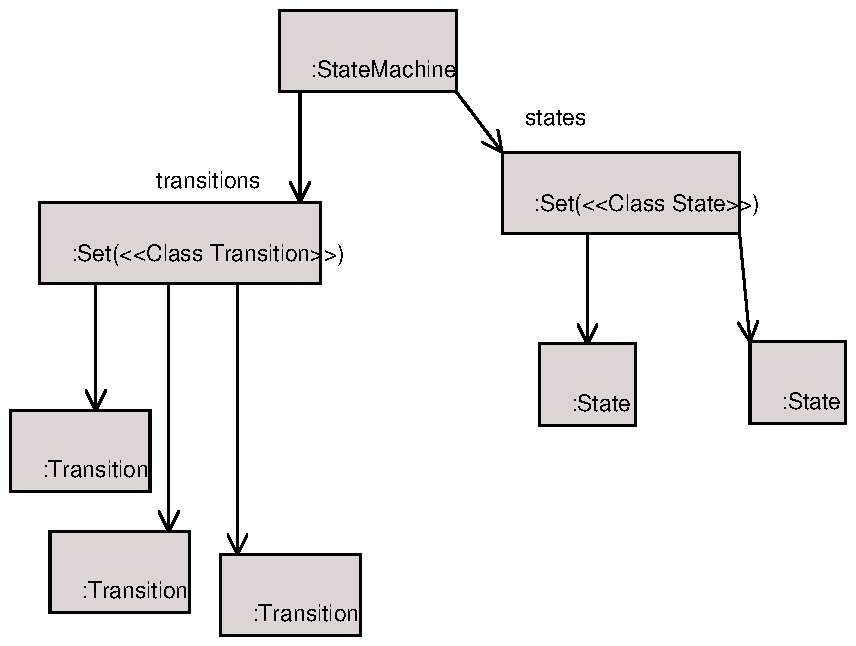
\includegraphics[width=11cm]{XMF/figures/snapshot.pdf}
\caption{A snapshot showing an instance of the statemachine
metamodel} \label{snapshotExample}
\end{center}
\end{figure}

Of course, because XMF provides an interpreter, instances of
models can be easily created and tested via its interpreter
console.

\subsection{Concrete Syntax}

The concrete syntax of a modelling language defines the notation
that is used to present models in the language. A notation may be
textual, or diagrammatical, or a mixture of both. A key part of
any metamodelling language is the ability to model both these
aspects in a platform independent way, and as a result facilitate
the rapid creation of parsers and diagram editors for a new
language.

\subsubsection{Textual Syntax}

XMF provides a generic parser language that can be used to model
the textual syntax of any language. This language, called XBNF
(the reader will be starting to see a pattern to our naming
conventions by now!) allows new textual constructs to be defined
that can be used as input to a model parser. These new constructs
to be defined as:


\begin{lstlisting}
@<NAME>
  <BODY>
end
\end{lstlisting}
\noindent where {\tt <NAME>} is the name of the construct and{\tt
<BODY>} is an XBNF expression.

An XBNF expression consists of a number of EBNF definitions within
which XOCL variables are embedded, followed by an XOCL expression.
When a construct is parsed, the XBNF expression is used to match
each parsed element with the variables. These variables can then
be used within the XOCL action to create instances of classes that
populate a model of the abstract syntax of a language.

Imagine that we wish to create a concrete syntax for the simple
StateMachine example. One part of this task would be to create a
concrete syntax for states. This might take the form:

\begin{lstlisting}
@State On
end

@State Off
end
\end{lstlisting}The following XBNF defines the syntax for parsing states and
populating instances of the class State.

\begin{lstlisting}
State ::= name = Name {[| State(name) |]}
\end{lstlisting}\noindent Now we have a new construct. When we type:

\begin{lstlisting}
@State X end
\end{lstlisting}\noindent we will get an instance of the class State named X.

\noindent Chapter \ref{concretechapter} will provide more detail
on the use of XBNF.

\subsubsection{Diagrammatical Syntax}

In order to model the diagrammatical syntax of a modelling
language, XMF provides a generic model of diagram elements such as
boxes, lines, etc, that can be tailored to support specific types
of diagrams. Bi-directional mappings are used to model the
relationship between a specific diagram model and the model of the
language's abstract syntax. This ensures that whenever changes are
made to a diagram, they are reflected in the model and vice versa.
By providing an interpreter (written in XMF) for displaying
instances of a diagrammatical syntax model, it is possible to
construct new diagram editors for a specific modelling language in
very short timescales. Chapter \ref{concretechapter} provides more
detail on this aspect.

\subsection{Mappings}

Chapter \ref{lddchapter} highlighted the fact that one important
use case of languages is to transform or relate them to other
languages. Mappings describe how models or programs in one
language are transformed or related to models or programs in
another. In order to describe these mappings, mapping languages
are required.

Two types of mapping languages are included in XMF: a
uni-directional pattern oriented mapping language called XMap, and
a bi-directional synchronisation language called XSync.

\subsubsection{Uni-directional Mappings}

XMap, is a declarative, executable language for expressing
uni-directional mappings that is based on pattern matching.

To illustrate the use of XMap, figure \ref{cppExample} shows a
simple model of {C++} classes which will be used as the target of a
mapping from a state machine.

\begin{figure}[htb]
\begin{center}
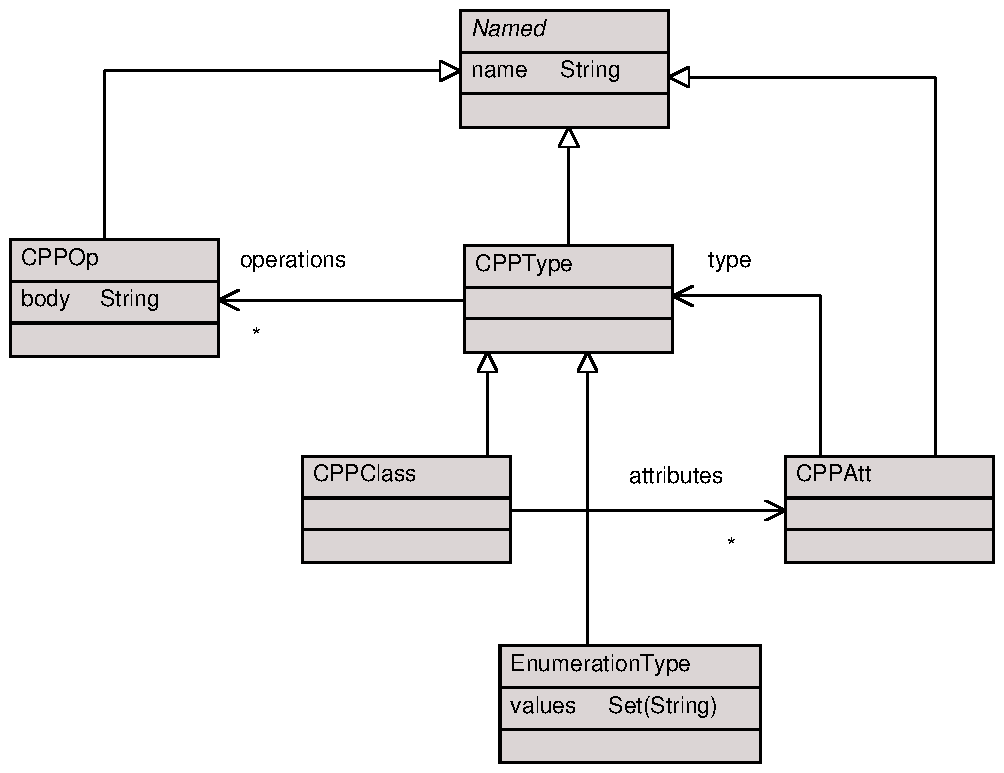
\includegraphics[width=11cm]{XMF/figures/cppSimple}
\caption{A simple model of C++ classes}
\label{cppExample}
\end{center}
\end{figure}

A {C++} class is a namespace for its attributes and operations
(methods). An attribute has a type, and for the purposes of this
example, its type may either be another class or an enumeration
type. An enumeration type has a value, which is the sequence of
strings in the enumeration. An operation has a name and a body,
which contains a simple string representation of the body of the
operation.

A mapping from from the StateMachine model in figure
\ref{classDiagram} to the {C++} in \ref{cppExample} can be
defined. This maps a StateMachine to a {C++} class, where each
state in the state machine is mapped to a value in an enumerated
type called STATE. Each transition in the state machine is mapped
to a {C++} operation with the same name and a body, which changes
the state attribute to the target of the transition.

The mapping can be modelled in XMap as shown in figure
\ref{cppmapping}.  The arrows represent mappings between elements
of the two languages. A mapping has a domain (or domains), which
is the input to the mapping, and a range, which is the output. The
first mapping, SM2Class, maps a state machine to a C++ class. The
second mapping, Transition2Op, maps a transition to an operation.

\begin{figure}[htb]
\begin{center}
\includegraphics[width=14cm]{XMF/figures/cppMapping}
\caption{A mapping between state machines and C++ classes}
\label{cppmapping}
\end{center}
\end{figure}

In order to describe the details of the mapping, XMap uses a
textual  mapping language based on pattern matching. Working
backwards, the definition of the mapping between a transition and
an operation is as follows:

\begin{lstlisting}
context Transition2Op
  @Clause Transition2Op
    StateMachines::Transition
      [sourceName = S,
       targetName = T]
    do
    CPP::Operation
      [name = S+T,
       body = B]
    where
      B = "state = " + T
  end
end
\end{lstlisting}A mapping consists of a collection of clauses, which are pattern
matches between source and target objects. Whenever a source object
is successfully matched to the input of the mapping, the resulting
object in the do expression is generated. Variables can be used
within clauses, and matched against values of slots in objects.
Because XMap builds on XOCL, XOCL expressions can also be used to
capture complex relationships between variables.

In this example, whenever the mapping is given a Transition with a
sourceName equal to the variable S and a targetName equal to T, it
will generate an instance of the class Operation, whose name is
equal to the concantenation of S and T, and whose body is equal to
the variable B. The where clause is used to define values of
variables, and it is used here to define the variable B to be
concatenation of the text "state = " with the target state name.
For instance, given a transition between the states "On" and
"Off", the resulting operation will have the name "OnOff" and the
body "state = Off". Note that it would be quite possible to model
a part of the syntax of {C++} expressions, and equate B with an
instance of an expression class.

The mapping between state machines and {C++} classes is shown below:


\begin{lstlisting}
 context SM2Class
   @Clause SM2Class
     StateMachines::StateMachine
       [states = S,
        transitions = TS]
     do
     CPP::CPPClass
       [attributes =
         Set{CPP::CPPAtt
           [name = "state",
            type = T]},
        operations = O]
     where
       T = CPP::EnumerationType
         [name = "STATE",
          values = S->collect(s | s.name)];
       O = TS->collect(t | Transition2Op(t))
  end
\end{lstlisting}
Here, a state machine with a set of states, S, and a set of
transitions, TS, is mapped to a {C++} class with a distinguised
attribute state of type T, and a set of operations, O. The value
of T is an EnumerationType whose name is ``STATE'' and whose
values are the names of the states in S. Finally, the transitions
are mapped to operations by iterating through the transitions in
TS and applying the Transition2Op mapping.

This mapping illustrates the power of patterns in being able to
match arbitrarily complex structures of objects. As shown by the
class CPPClass, objects may be matched with nested objects to any
depth. It also shows the necessity of a rich expression language
like OCL for capturing the complex navigation expressions that are
often encountered when constructing mappings.

\subsubsection{Synchronised Mappings}

While it is common to want to translate from one language to
another, there is also a requirement to keep different models in
sync. For example, an abstract syntax model will need to be kept
in sync with a model of its concrete syntax, or a model may need
to be synchronised with code. To achieve this, XMF provides a
bi-directional mapping language called XSync. This enables rules
to be defined that state how models at either end of a mapping
must change in response to changes at the other end, thus
providing a declarative language for synchronisation. This
language will be explored in greater detail in chapter
\ref{mappingchapter}.

\section{XMF Architecture}

As outlined in the previous chapter, XMF follows the golden braid
metamodel architecture, and therefore is defined in its own
language. Understanding the architecture of XMF is important for
many reasons. Firstly, it provides a good example of a language
definition in its own right - the fact that XMF is self describing
makes a strong statement about the expressibility of the language.
Secondly, XMF acts as a foundation for many other metamodel
definitions. For instance, it can be viewed as a subset of the UML
metamodel, and many other types of modelling languages can also be
viewed as extensions of the core architecture.

Figure \ref{XMFOverview} shows the key components of the XMF
architecture. At the heart of XMF is the XCore metamodel. This
provides the core modelling concepts of the metamodelling language
(as described in section \ref{coreconcepts}). This metamodel also
provides a framework for language extension (a topic discussed in
more detail in chapter \ref{langchapter}). Around it, sit the
metamodels for the OCL, XOCL, XBNF, XMap and XSync languages.

The classes and relationships in these metamodels correspond
precisely to the modelling features that have been used in this
chapter. For example, the package and classes shown in the
StateMachine abstract syntax model in figure \ref{classDiagram}
are concrete syntax representations of instances of the classes
XCore::Package and XCore::Class. Expressions in a concrete syntax
model are themselves instance of XBNF::Grammar, and so on.

\begin{figure}[htb]
\begin{center}
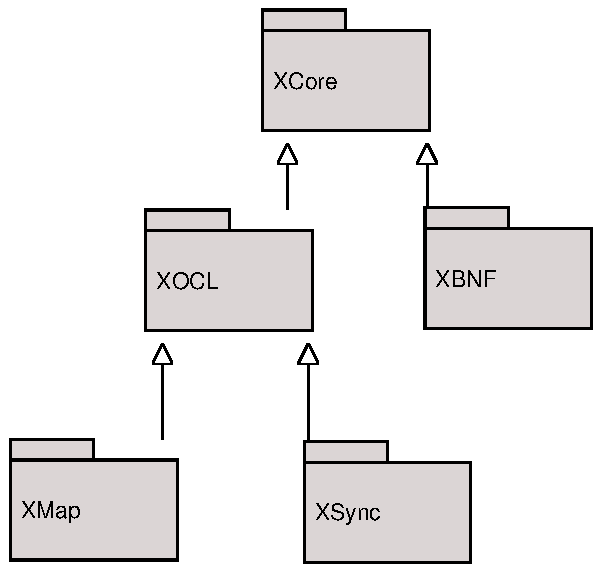
\includegraphics[height=8cm]{XMF/figures/arch.pdf}
\caption{Overview of XMF Architecture} \label{XMFOverview}
\end{center}
\end{figure}

\subsection{XCore Metamodel}

As shown in figure \ref{coreMetamodel}, the classes that are
defined in the XCore metamodel provide the core modelling concepts
used in XMF such as Class and Package. As we discuss metamodelling
in more detail in later chapters, many of the features of this
metamodel will discussed in detail.

\begin{figure}[htb]
\begin{center}
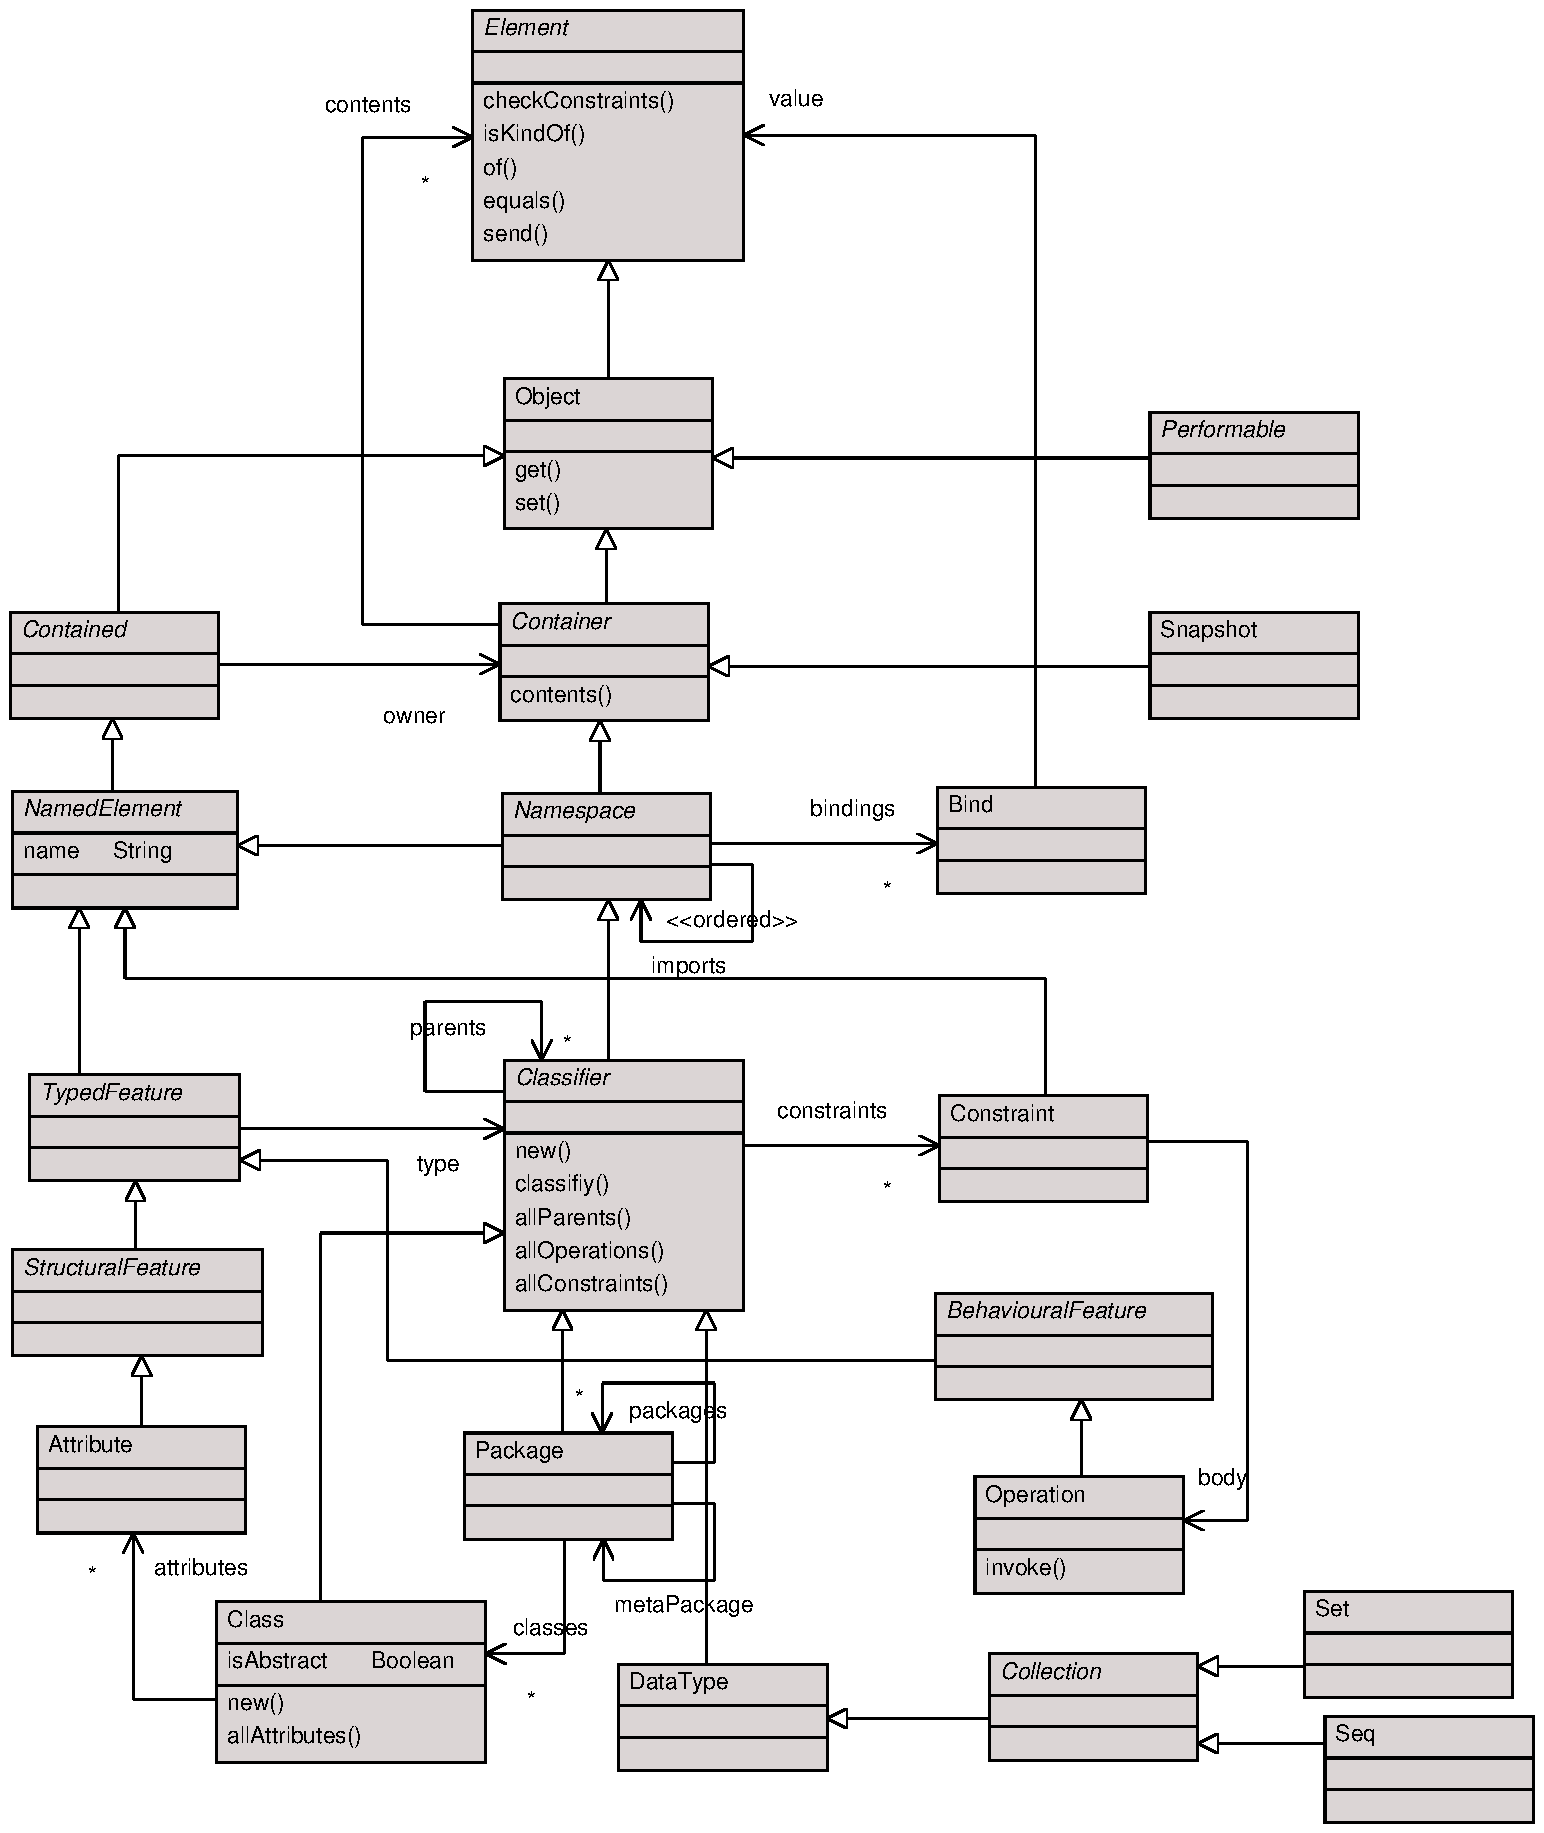
\includegraphics[height=21cm]{XMF/figures/xcore.pdf}
\caption{The XCore Metamodel} \label{coreMetamodel}
\end{center}
\end{figure}

\noindent There are however, some key parts of this model that are
worth pointing out here:

\begin{description}
\item[Elements and Objects] The most fundamental modelling
concepts in XMF are elements and objects. Elements are the root of
all modelling concepts, in other words, every type of modelling
concept in XMF is an element. All elements are instances of a
classifier. Elements do not have structure or state. Objects on
the other hand are elements that encapsulate data values - called
slots in XMF. An object's slots must conform to the name and type
of the attributes of the class it is an instance of.
\item[Performable] The performable class represents the root of
all modellng concepts that can be evaluated in the context of an
environment (a collection of variable bindings) to return a
result. An OCL expression is a good example of a performable
concept. \item[Classification] In XMF some types of modelling
elements are modelled as Classifiers. A Classifier is an element
that can be instantiated via the new() operation to create new
instances. Good examples of these elements are classes and
datatypes, which can be instantiated to create objects and
datavalues. All elements have an of() operation, which returns the
classifier that the element was instantiated from. For example the
objects statemachine1, statemachine2 will return the class
StateMachine while the object fido might return the class Dog.
\item[Reflection] An important property of all XMF models is that
classes are also objects. This apparently strange assumption means
that classes can also be viewed as instances of classes. This
capability is an important one, as it enables any operation that
can be carried out on an object such as executing its operations,
or mapping it to another object can also be applied to classes.
\item[XOCL] The XOCL class is an extension of OCL, and is the root
of all imperative expressions that can change the state of a model
(not shown here). \item[Snapshot] A snapshot is a collection of
elements, and may therefore include any type of element that is
available in XMF. \item[Grammar] A grammar can be evaluated in the
context of sequence of tokens to generate an instance of a model.
\end{description}

In addition, the XCore metamodel defines a number of abstract
classes that provide a framework for language design. This
framework will be discussed in greater detail in chapter
\ref{langchapter}.

\section{Relationship to Existing Metamodelling Languages}
\label{differences}

The requirement to be able to construct metamodels is not a new
one, and not surprisingly a variety of languages have been
proposed as metamodelling languages. The most notable of these are
UML and the MOF (the Meta Object Facility). The MOF is the
standard language for capturing meta-data, and goes further than
the UML in meeting the requirements of a metamodelling language.
Nevertheless, whilst the MOF provides many of the features
necessary to define metamodels, there are a number of crucial
areas in which it needs to be extended.

\begin{itemize}
\item The MOF does not explicitly support executable metamodelling
in a platform independent way. Although it does provide OCL, this
does not support the construction of operations that change the
state of a model. An alternative might be to use the Action
semantics. This is a platform independent language for executing
models that is currently a part of the the UML 1.5 metamodel.
There are a number of problems with this language however.
Firstly, it does not have a concrete syntax, which has slowed its
adoption. Secondly, it is a complex language that includes many
constructs that are not relevant to metamodelling, such as
concurrent actions. Whilst work is ongoing to resolve the first
issue, XOCL resolves both by the minimal extension of OCL,
resulting in a powerful executable metaprogramming language. \item
The MOF does not support an extensible grammar language. This is
important in being able to model new concrete syntax grammars in
MOF. \item The MOF currently is not defined fully in terms of
itself. Its semantics and syntax are stated in a form (a mixture
of OCL, and informal English) that prevents it from being
completely self describing and self supporting. \item The MOF
currently does not support mapping languages such as the XMap and
XSync languages described above. Work is currently proceeding on
an extension to MOF called QVT (Queries, Views, Transformations),
which aims to define a language for doing uni-directional
mappings, but it is unclear at this stage whether it will support
all the capabilities of XMap in the short to medium term. There is
unlikely to be support for synchronised mappings in the near
future.
\end{itemize}

XMF aims to provide these extensions in the most concise and
minimal fashion necessary to support precise, semantically rich
metamodelling.

\section{Conclusion}

This chapter has described some of the essential features of XMF,
an extended MOF like facility that provides the ability to define
platform independent metamodels of semantically rich languages.
These facilities will be used throughout the rest of this book to
illustrate the metamodelling process in greater detail.
